\chapter{Síntesis de imágenes de radiointerferometría}
\label{cap:imagesynthesisinterferometry}

\section{Atacama Large Millimeter-Submillimeter Array}

El Atacama Large Millimeter-Submillimeter Array (ALMA) es un radiointerferómetro compuesto de 66 antenas de alta precisión que operan a un ancho rango de frecuencias milimétricas y submilimétricas. Cincuenta de estas antenas miden 12 metros de diámetro y son utilizadas para síntesis de imágenes de alta resolución. Por otra parte, esto es complementado por el \textit{Atacama Compact Array} también llamado \textit{Morita Array} compuesto por doce antenas de 7 metros de diámetro y por otras 4 antenas de 12 metros diámetro que sirve para muestrear estructuraS de gran escala que no son bien muestreadas por las demás antenas de 12 metros. Además, todas las antenas se clasifican en tres tipos:

\begin{itemize}
\item \textbf{AEM (DA) 12m}: Estas antenas fueron ensambladas antes de llegar a Chile, por lo tanto, llegaron en pocas piezas. Estas antenas están manejadas por motores lineales, es decir, imanes que proveen el movimiento sin que exista un contacto entre las partes.
\item \textbf{Vertex (DV) 12m}: La estructura que sostiene al platillo está hecha de plástico reforzado con fibra de carbón, lo cual es importante debido a las duras condiciones de 5.000 metros de altura.
\item \textbf{MELCO (PM) 12m y 7m}: Estas antenas también poseen motores lineales además de una conducción en tres direcciones (altura, de lado a lado y de arriba a abajo), para seguir suavemente la fuente durante la observación.
\end{itemize}

El conjunto de antenas está ubicado en el llano Chajnantor a 5.000 metros sobre el nivel del mar, un sitio que ofrece un cielo claro y un aire seco, una condición ambiental requerida para observar ondas milimétricas y submilimétricas.

La distribución de las antenas cede paso a lo que es llamado \textit{baseline} o distancia entre un par de antenas, que van desde 15 Km. hasta 16 Km. aproximadamente. Tanto la distribución como la distancia entre éstas es crucial en la determinación de la calidad de la imagen y la resolución de ALMA. Esto debido a que si el conjunto de antenas está distribuido de forma extendida dará como resultado una alta resolución espacial, en cambio, si la distribución es compacta, el resultado será una mejor sensibilidad para fuentes extendidas.

A continuación, la Figura \ref{fig:almaarray1} muestra la distribución de antenas para el muestreo del objeto HLTauri en banda 6. Además la Figura \ref{fig:almaarray2} muestra el centro de la primera figura en donde se puede visualizar una gran concentración de antenas. Además, se puede ver que cada antena posee un identificador (DA, DV o PM) dando a conocer los tipos de antena que están siendo utilizados para el muestreo. Es importante que cada antena tiene una coordenada $X$ que apunta hacia al este geográfico y una coordenada $Y$ que apunta al norte geográfico.

\begin{figure}[h!]
\centering
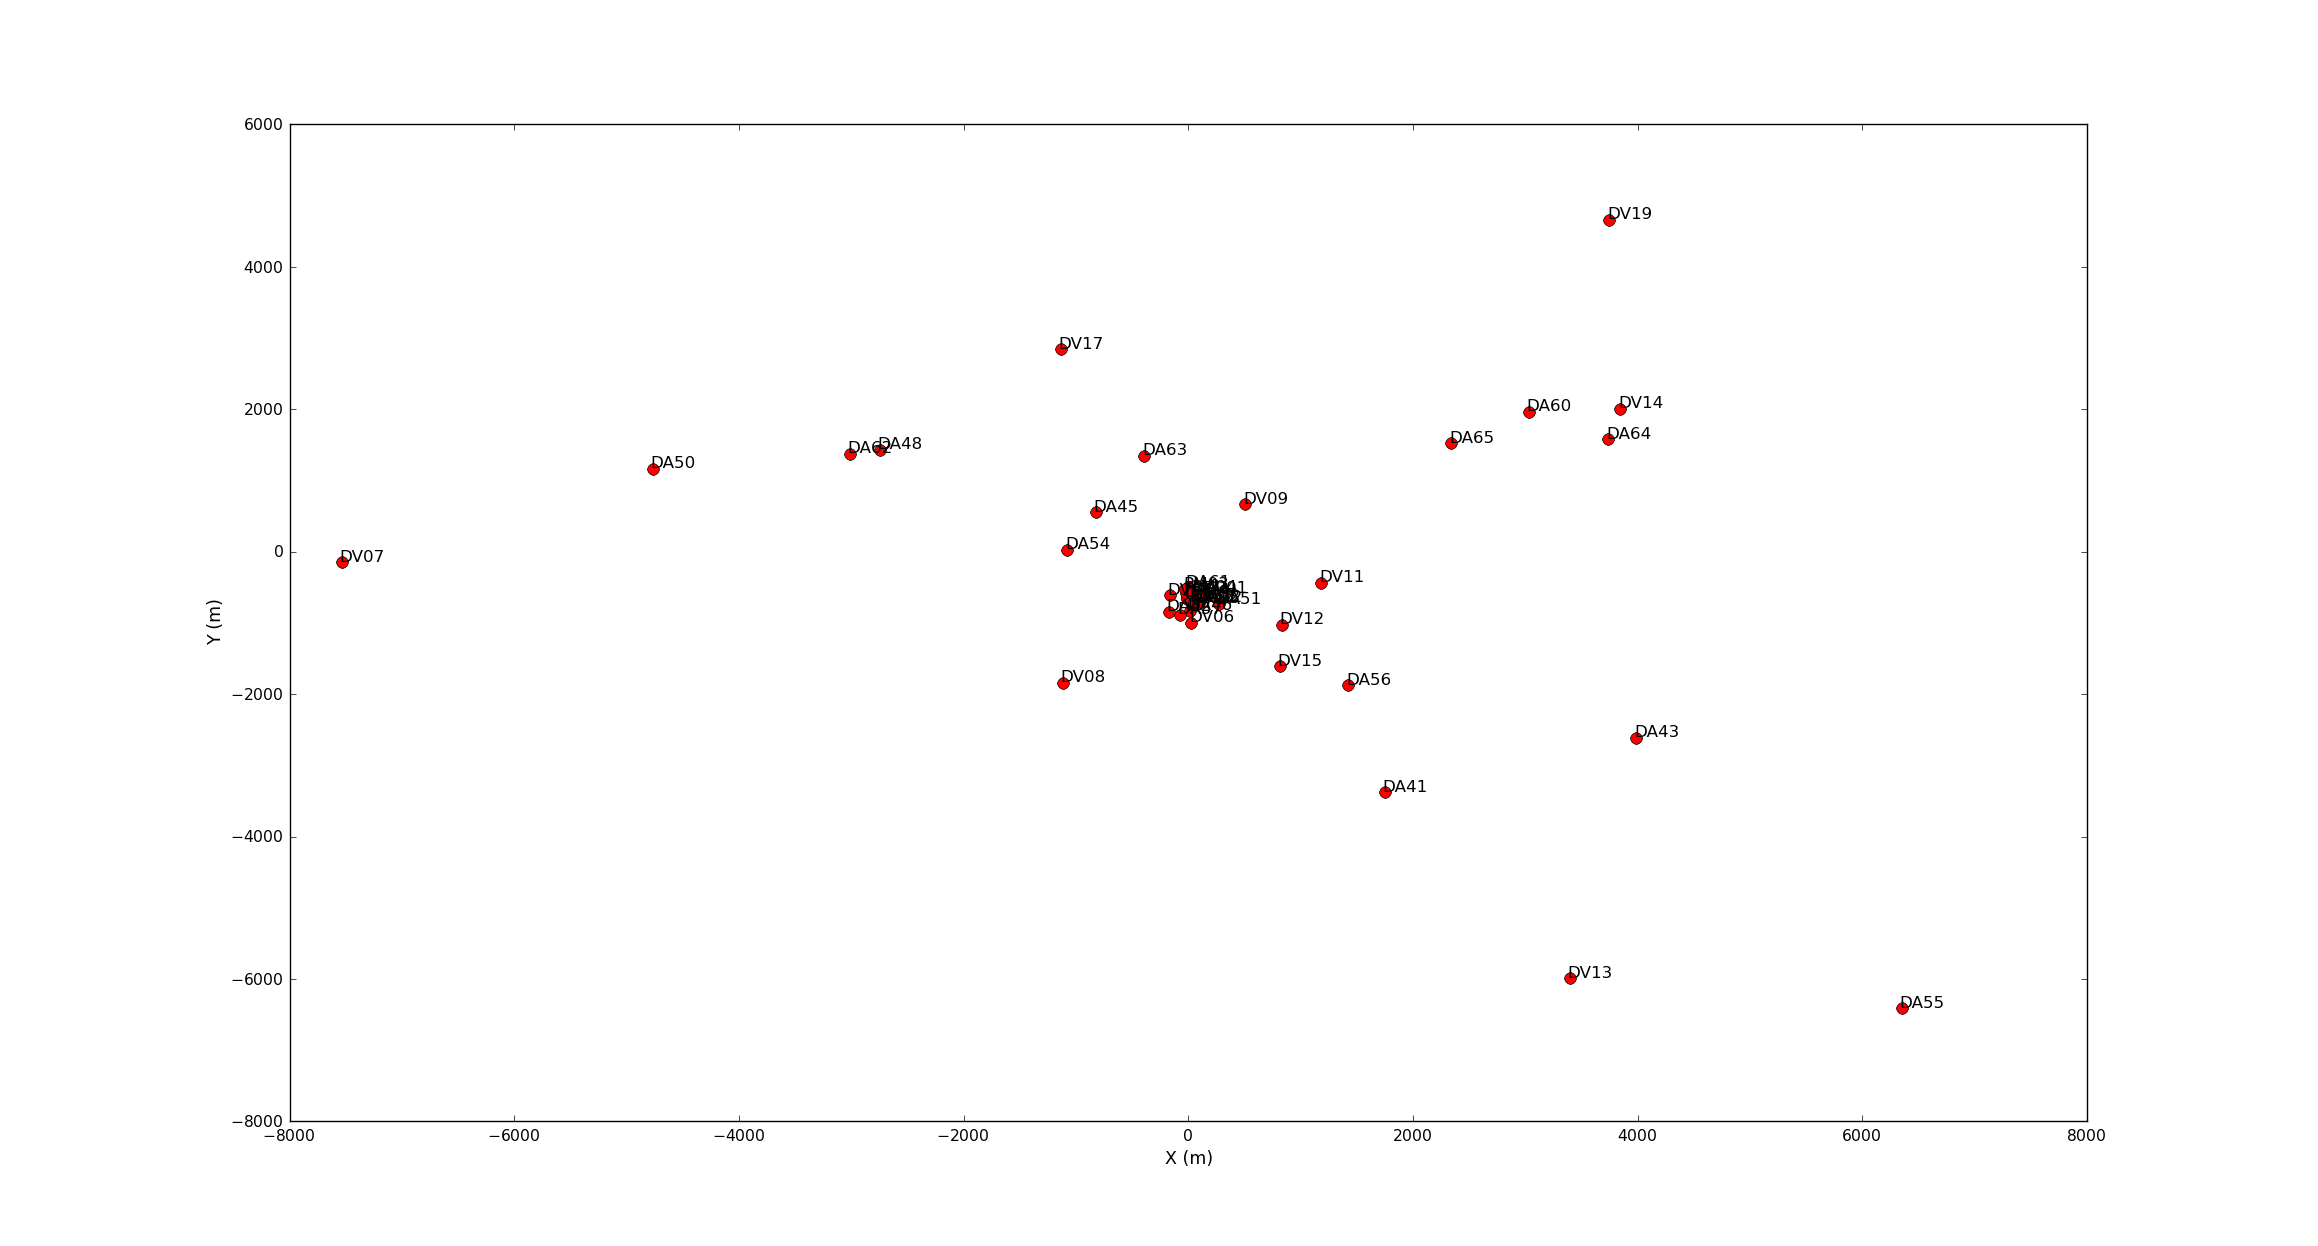
\includegraphics[scale=0.25]{images/HLTau_B6antennas1.png}
\caption{Distribución de antenas para el muestro del objeto HLTauri en banda 6. Fuente: Elaboración propia.}
\label{fig:almaarray1}
\end{figure}

\begin{figure}[h!]
\centering
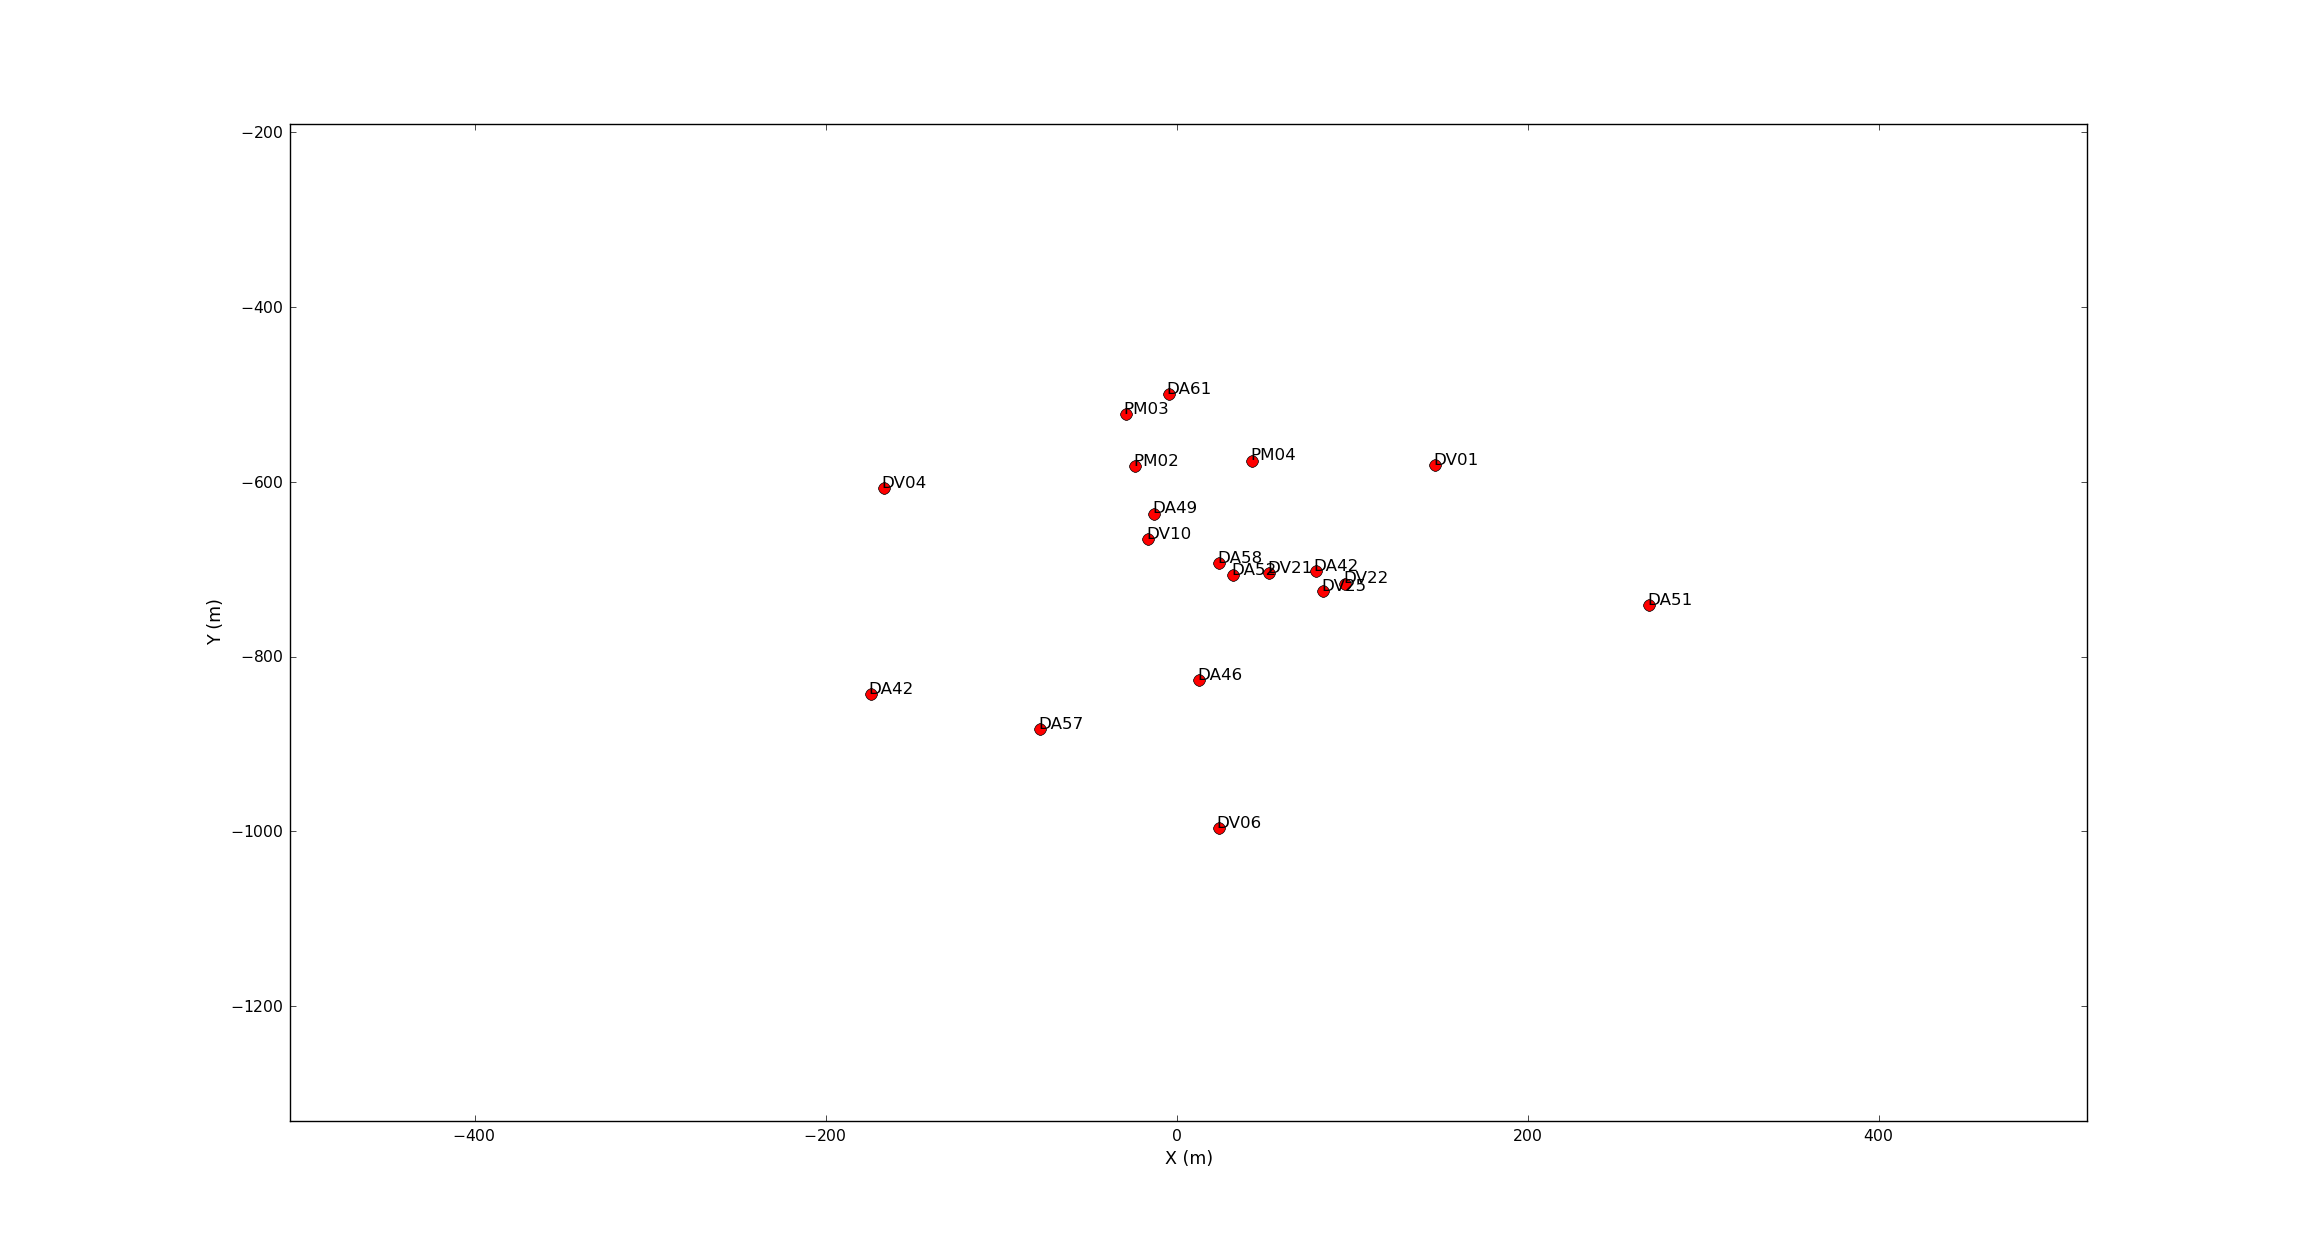
\includegraphics[scale=0.25]{images/HLTau_B6antennasCenter.png}
\caption{Centro de la distribución de antenas para el muestro del objeto HLTauri en banda 6. Fuente: Elaboración propia.}
\label{fig:almaarray2}
\end{figure}

Variados sistemas de coordenadas son usados para especificar la posiciones de las antenas en un \textit{array}. Uno de los sistemas usa coordenadas ecuatoriales horarias, es decir un ángulo horario $H$ y la declinación $\delta$. El ángulo $H$ se mide entre cero y 360 grados o entre cero y 24 horas sidéreas. Por lo tanto, a cada hora le corresponden $360°/24 = 15°$. Además, se mide a partir de la intersección del meridiano local con el ecuador. Su extremo es la intersección del meridiano que pasa por el objeto a observar ($S$) con el ecuador. 

Por otra parte, la declinación es el ángulo medido sobre el meridiano que para por la estrella u objeto a observar, entre el ecuador la dirección de éste, sus valores están comprendidos entre cero y $+90°$ para los astros del hemisferio norte, y entre cero y $-90°$ para los astros del hemisferio sur \citep{astroelemental}.

En la Figura \ref{fig:ecuatorial2} se muestra el sistema de coordenadas ecuatoriales usado para arreglos de antenas terrestres. Se puede ver un sistema cartesiano donde $X$ e $Y$ están en un plano paralelo al ecuador de la tierra, donde $X$ es parte del plano meridiano (definido como el plano que pasa por los polos de la tierra y el punto de referencia del arreglo de antenas, $Y$ se mide hacia el este, y Z hacia el polo norte \citep{libroAstro}. En términos de ángulo horario $H$ y declinación $\delta$, las coordenadas $(X,Y,Z)$ se miden como lo muestra la Figura \ref{fig:ecuatorial1}.
%$H$ se mide a partir del punto $Q$ (intersección del meridiano del lugar con el Ecuador) en sentido horario. Su extremo es el punto $A$ (intersección del meridiano que pasa por el objeto a observar con el Ecuador). El ángulo $H$ se mide entre cero y 360 grados o entre cero y 24 horas sidéreas. Por lo tanto, a cada hora le corresponden $360°/24 = 15°$. Por otro lado, la declinación es el ángulo medido sobre el meridiano que pasa por la estrella u objeto a observar, entre el Ecuador y la dirección de éste. Es decir, el ángulo correspondiente al arco $AE$. Sus valores están comprendidos entre cero y $+90°$ para los astros del hemisferio Norte, y entre cero y $-90°$ para los astros del hemisferio Sur \citep{astroelemental}.
\begin{figure}[h!]
\centering
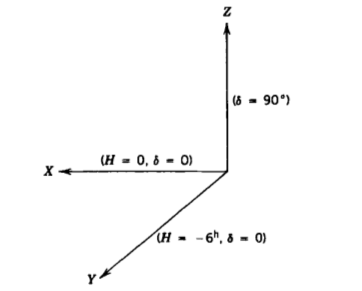
\includegraphics[scale=0.6]{images/ecuatorial1.png}
\caption{Sistema de coordenadas $(X,Y,Z)$ y la dirección de los ejes en términos de ángulo horario $H$ y declinación $\delta$. Fuente: \citep{libroAstro}}.
\label{fig:ecuatorial1}
\end{figure}

\begin{figure}[h!]
\centering
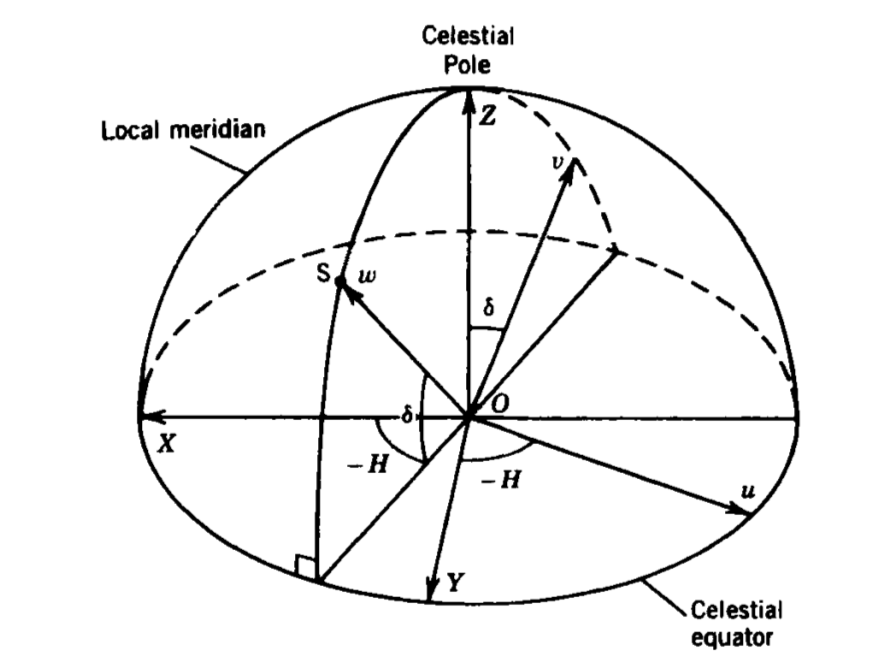
\includegraphics[scale=0.3]{images/ecuatorial2.png}
\caption{%Coordenadas ecuatoriales horarias.
Relación entre los sistemas de coordenadas $(X,Y,Z)$ y $(u,v,w)$. El sistema $(u,v,w)$ está definido por la observación en la dirección del punto $S$, el cual tiene un ángulo horario $H$ y una declicación $\delta$. Como $S$ está en el la mitad del hemisferio este, $H$ es negativo (sentido anti-horario). Fuente: \citep{libroAstro}}.
\label{fig:ecuatorial2}
\end{figure}

Es importante destacar que las estrellas describen en su movimiento diurno aparente, círculos paralelos de la Esfera Celeste y tienen por lo tanto declinación constante. Sin embargo, no sucede lo mismo con el Sol, la Luna o los planetas.

Teniendo esto en consideración, una coordenada del plano $(u,v)$ que genera un baseline está dada por:

\begin{equation}
\begin{bmatrix}
u\\
v\\
w
\end{bmatrix}
=
\begin{bmatrix}
\sin{H} & \cos{H} & 0\\
-\sin{\delta}\cos{H} & \sin{\delta}\sin{H} & \cos{\delta}\\
\cos{\delta}\cos{H} & -\cos{\delta}\sin{H} & \sin{\delta}
\end{bmatrix}
\begin{bmatrix}
X\\
Y\\
Z
\end{bmatrix}
\label{eq:uvw}
\end{equation}


Donde las coordenadas en el sistema $(X,Y,Z)$ están dadas por:

\begin{equation}
\begin{bmatrix}
X\\
Y\\
Z
\end{bmatrix}
=
D
\begin{bmatrix}
\cos{d}\cos{h}\\
-\cos{d}\sin{h}\\
\sin{d}
\end{bmatrix}
\label{eq:XYZ}
\end{equation} 

Aquí, $(H, \delta)$ son el ángulo horario y la declinación de la posición de fase de referencia. Por otra parte es importante especificar el vector del \textit{baseline} en términos de su longitud $D$ y el ángulo horario y declinación $(h,d)$ de la intersección de la dirección del \textit{baseline} con el norte celestial. Reemplazando la Ecuación \ref{eq:XYZ} en \ref{eq:uvw} y usando identidades trigonométricas se tiene que:


\begin{equation}
\begin{bmatrix}
u\\
v\\
w
\end{bmatrix}
=
D
\begin{bmatrix}
\cos{d}\sin{(H-h)}\\
\sin{d}\cos{\delta}-\cos{d}\sin{\delta}\cos{(H-h)}\\
\sin{d}\sin{\delta}+\cos{d}\cos{\delta}\cos{(H-h)}
\end{bmatrix}
\label{eq:uvw2}
\end{equation} 

Si bien el sistema $(D,h,d)$ era el más usado con instrumentos que sólo consistían en dos antenas. Cuando se tiene dos antenas o más, la práctica usual es utilizar el sistema de coordenadas horizontales para determinar la elevación $\mathscr{E}$, el \textit{azimuth} $\mathscr{A}$ y el largo del baseline $D$.

\begin{figure}[h!]
\centering
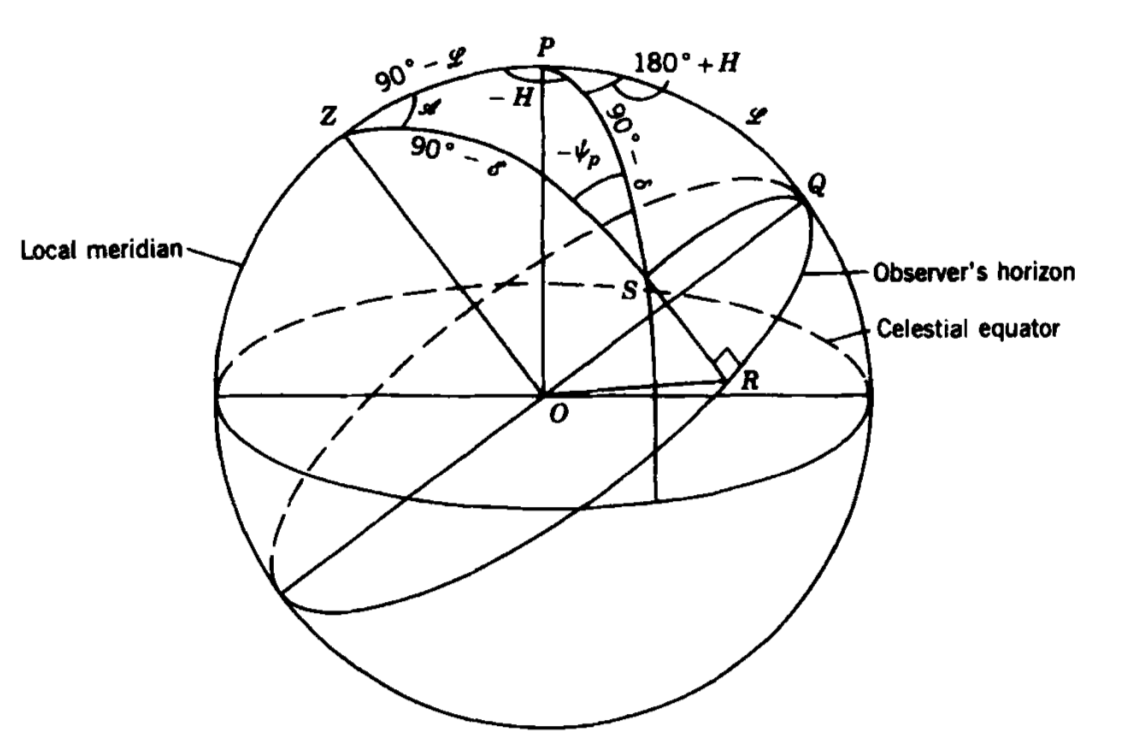
\includegraphics[scale=0.3]{images/horizontales.png}
\caption{Relación entre coordenadas horizontales y coordenadas ecuatoriales horarias. Fuente: \citep{libroAstro}}
\label{fig:horizontal}
\end{figure}

%%%%Explicar el sistema de coordenadas horizontales
El plano de referencia es el horizonte, perpendicular a la vertical del lugar de observación que pasa por el centro de la Tierra. $Z$ es el \textit{zenith} del observador y es la parte superior (más próximo al polo norte $P$) del plano vertical perpendicular al plano de observación. Por otra parte, el meridiano del lugar que pasa por el \textit{zenith}, corta al horizonte en una recta llamada meridiana que determina la dirección Norte-Sur. En este caso $Q$ indica el la dirección Norte, y luego mirando hacia éste, el Este queda a la derecha y el Oeste a la izquierda. Se llama \textit{azimuth} al ángulo $\mathscr{A}$ medido de Norte a Este en sentido anti-horario. Además, se llama elevación al ángulo $\mathscr{E}$ formado por la dirección de la fuente $S$ con el plano del horizonte.

Las fórmulas de conversión de coordenadas derivan de la aplicación de las reglas de seno y coseno para triángulos esféricos en la Figura \ref{fig:horizontal}. Por lo tanto para un observador a una latitud $\mathscr{L}$ se tiene que:

\begin{align}
\sin{d} &= \sin{\mathscr{L}}\sin{\mathscr{E}}+\cos{\mathscr{L}}\cos{\mathscr{E}}\cos{\mathscr{A}} \nonumber\\
\cos{d}\cos{h} &= \cos{\mathscr{L}}\sin{\mathscr{E}} - \sin{\mathscr{L}}\cos{\mathscr{E}}\cos{\mathscr{A}}\\
\cos{d}\sin{h} &= -\cos{\mathscr{E}}\sin{\mathscr{A}} \nonumber
\label{eq:transformation}
\end{align}

Reemplazando en la Ecuación \ref{eq:XYZ} se tiene:

\begin{equation}
\begin{bmatrix}
X\\
Y\\
Z
\end{bmatrix}
=
D
\begin{bmatrix}
\cos{\mathscr{L}}\sin{\mathscr{E}}-\sin{\mathscr{L}}\cos{\mathscr{E}}\cos{\mathscr{A}}\\
\cos{\mathscr{E}}\sin{\mathscr{A}}\\
\sin{\mathscr{L}}\sin{\mathscr{E}}+\cos{\mathscr{L}}\cos{\mathscr{E}}\cos{\mathscr{A}}
\end{bmatrix}
\end{equation}


Por otra parte, si se quisiera proyectar el plano $(u,v)$ en la Figura \ref{fig:ecuatorial2} bastaría que hicieramos $H=0$ en la ecuación \ref{eq:uvw} o \ref{eq:uvw2}, con esto se forma una ecuación de la elipse en el plano $(u,v)$ de la forma:

\begin{equation}
\frac{u^2}{(\sqrt{X^{2}+Y^{2}})^2}+\frac{(v-Z\cos{\delta})^2}{(\sin{\delta}\sqrt{X^{2}+Y^{2}})^2} = 1
\label{eq:elipse}
\end{equation}

Si se analiza la ecuación \ref{eq:elipse} es posible notar que su centro está en $(u,v)=(0,Z\cos{\delta})$, su eje semimayor se encuentra en $\sqrt{X^{2}+Y^{2}}$ y su eje semimenor en $\sin{\delta}\sqrt{X^{2}+Y^{2}}$. Este arco trazado durante la observación depende del \textit{azimuth}, la elevación y la latitud del \textit{baseline}; la declinación de la fuente, y el rango de ángulo horario que se cubre como se muestra en la Figura \ref{fig:uvplane2}. Además, como una de las propiedades de la transformada de Fourier es la simetría Hermitiana $V(u,v)=V(-u,-v)$, el correlacionador devuelve como salida el valor de la visibilidad en dos puntos en el plano $(u,v)$ como se muestra en la Figura \ref{fig:uvplane1}.

\begin{figure}[h!]
\centering
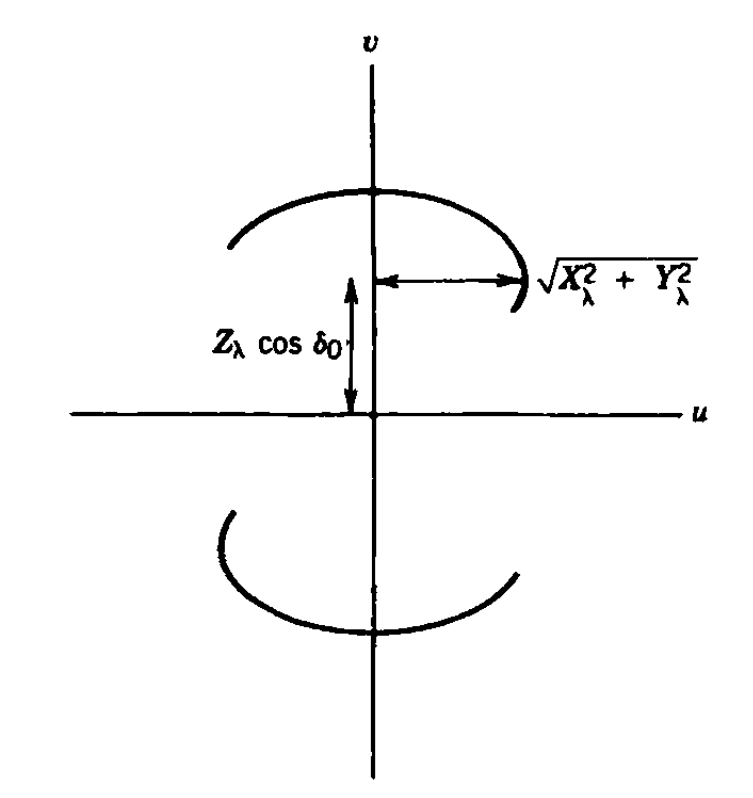
\includegraphics[scale=0.3]{images/uvplane1.png}
\caption{Centro y eje semimayor de la elipse (Ecuación \ref{eq:elipse}). Fuente: \citep{libroAstro}}
\label{fig:uvplane1}
\end{figure}

\begin{figure}[h!]
\centering
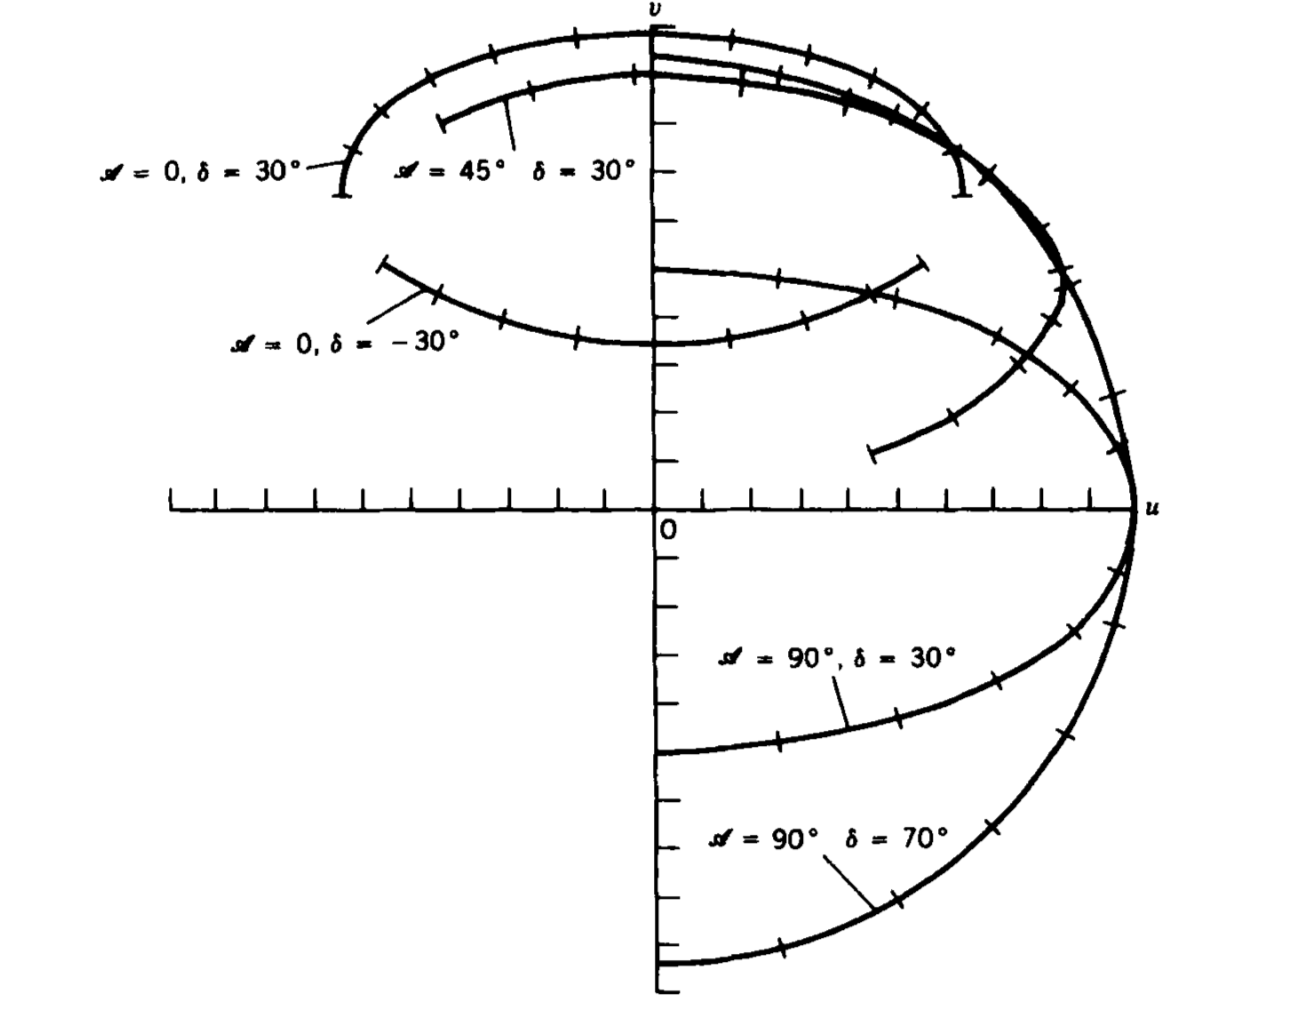
\includegraphics[scale=0.3]{images/uvplane2.png}
\caption{Elipses muestreadas con diferentes parámetros en el plano $(u,v)$. Fuente: \citep{libroAstro}}
\label{fig:uvplane2}
\end{figure}



\clearpage

Por otro lado, cada antena contiene un receptor (también llamado \textit{Front-end}) que permite que las éstas capten información en diez bandas de frecuencia diferentes. Para ello cada antena está equipada con un criostato y su criorefrigerador adjunto. Estos criostatos contienen receptores que están montados y pueden ser reemplazados de forma fácil. En la tabla \ref{tab:bands} se adjuntan los datos de las distintas bandas de frecuencia que ALMA puede cubrir gracias a su front-end.


\begin{table}[h!]
\centering
\ra{1.2}
\begin{tabular}{@{}rcrrcr@{}} 
\toprule
 \multicolumn{1}{c}{{\bf Banda}} & \phantom{a} & \multicolumn{2}{c}{{\bf Rango de frecuencia (GHz)}}  & \multicolumn{1}{c}{{\bf Temperatura (K)}} \\
 \midrule
 1   && 31 - 45 &&  26\\
 2   && 67 - 90 &&  47\\    
 3  && 84 - 116 &&  60\\
 4  && 125 - 163 &&  82\\
 5  && 162 - 211 &&  105\\
 6  && 211 - 275 &&  136\\
 7  && 275 - 373 &&  219\\
 8  && 385 - 500 &&  292\\
 9  && 602 - 720 &&  261\\
 10  && 787 - 950 &&  344\\
 \toprule
\end{tabular}
\caption{Las 10 Bandas de frecuencia de ALMA}
\label{tab:bands}
\end{table}

Por ejemplo, la estrella HLTauri ha sido muestreada en las bandas 3, 6 y 7. En la Figura \ref{fig:HLTau-total} es posible apreciar cada uno de los planos $(u,v)$ formados en cada muestreo.


\begin{figure}[h!]
\centering
\subfloat[Banda 3]{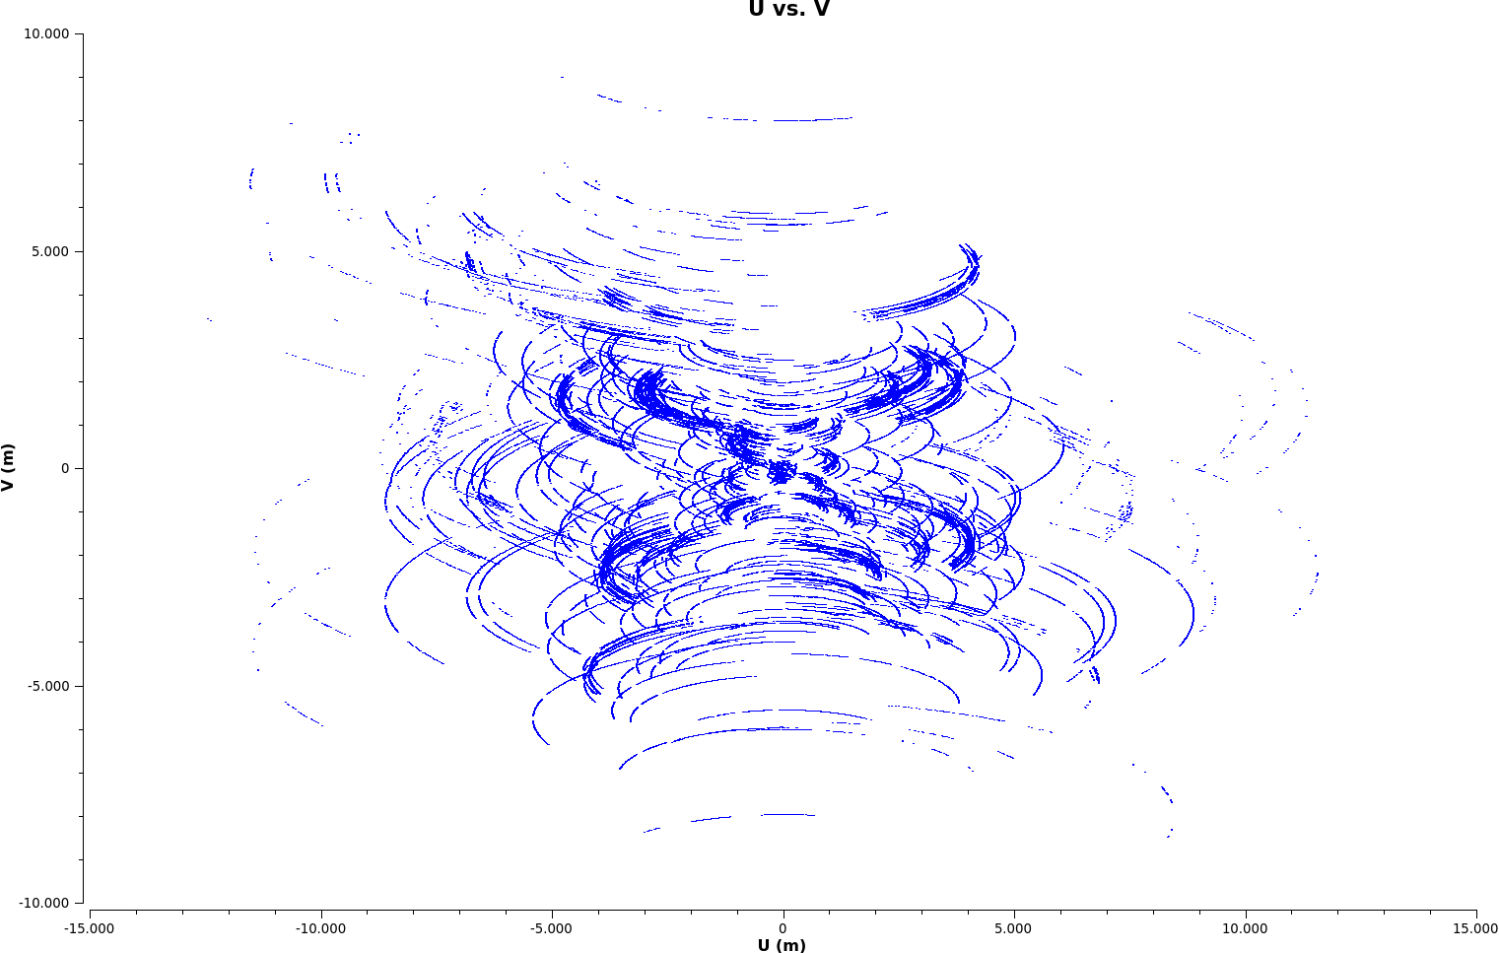
\includegraphics[scale=0.15]{images/HLTau_B3total.png}}%
\subfloat[Banda 6]{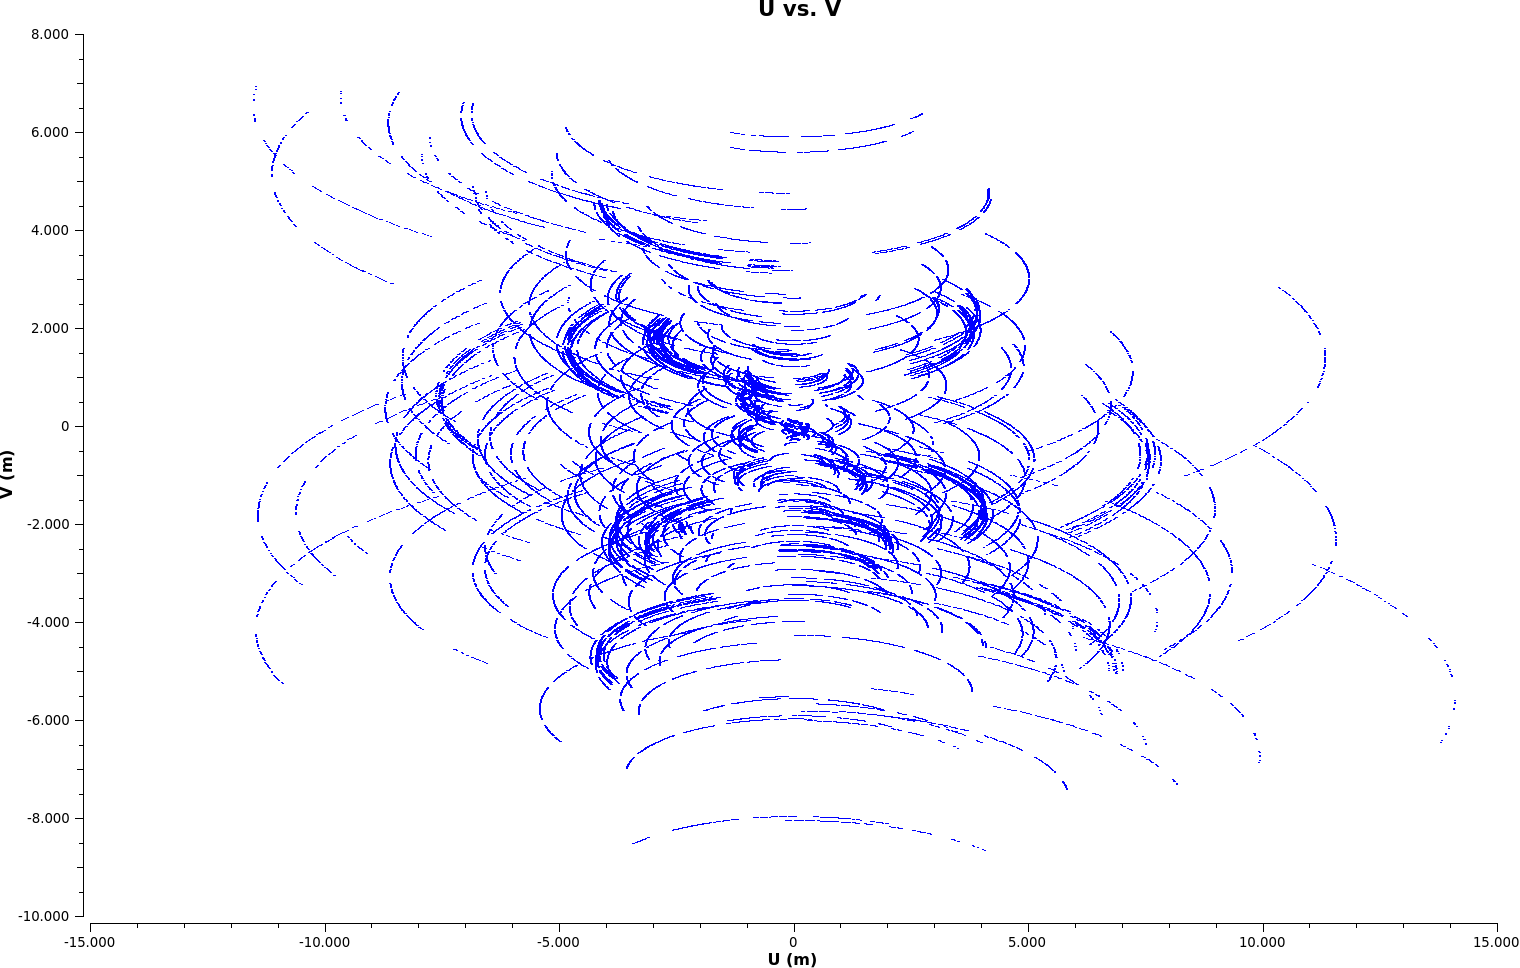
\includegraphics[scale=0.15]{images/HLTau_B6total.png}}\\
\subfloat[Banda 7]{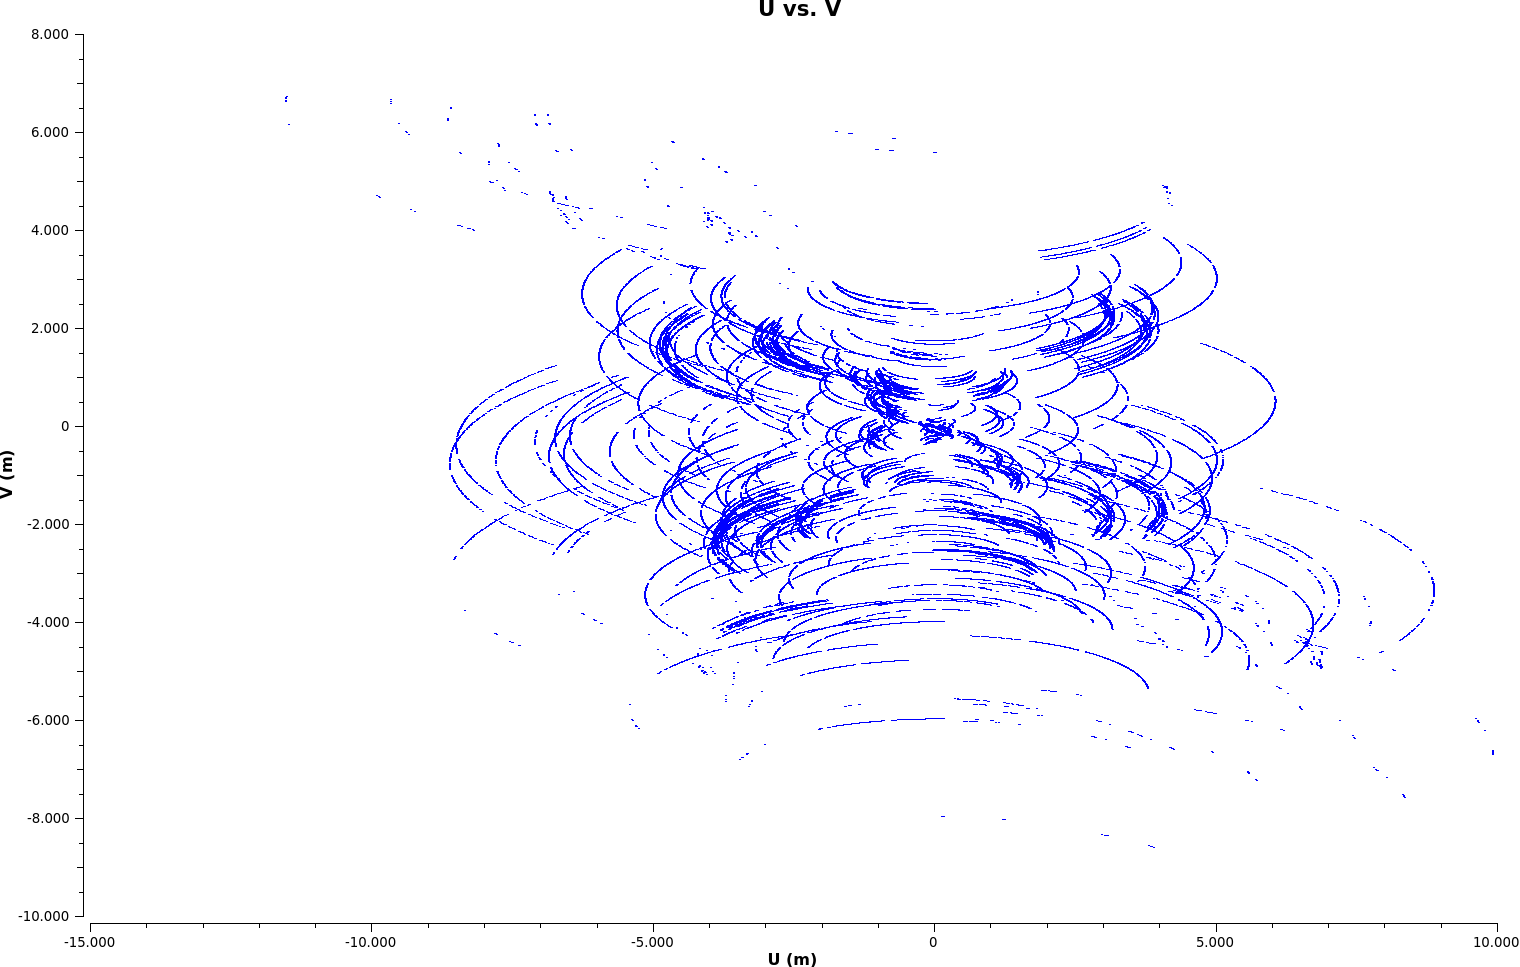
\includegraphics[scale=0.15]{images/HLTau_B7total.png}}%
\caption{Plano $(u,v)$ del objeto HLTauri (HLTau) en diferentes bandas. Fuente: Elaboración propia}
\label{fig:HLTau-total}
\end{figure}

Es importante destacar que los datos muestreados en una banda se separan en \textit{spectral windows} que son espectros contiguos cuyas frecuencia están uniformemente espaciadas con anchos de banda desde 58.6 MHz hasta 1.875 GHz \citep{alma-handbook}. Asimismo, cada \textit{spectral window} se divide uniformemente en canales. Es posible visualizar esto en la Figura \ref{fig:division}, en donde se ha puesto como ejemplo el muestreo del objeto HL-Tauri.

\begin{figure}[h!]
\centering
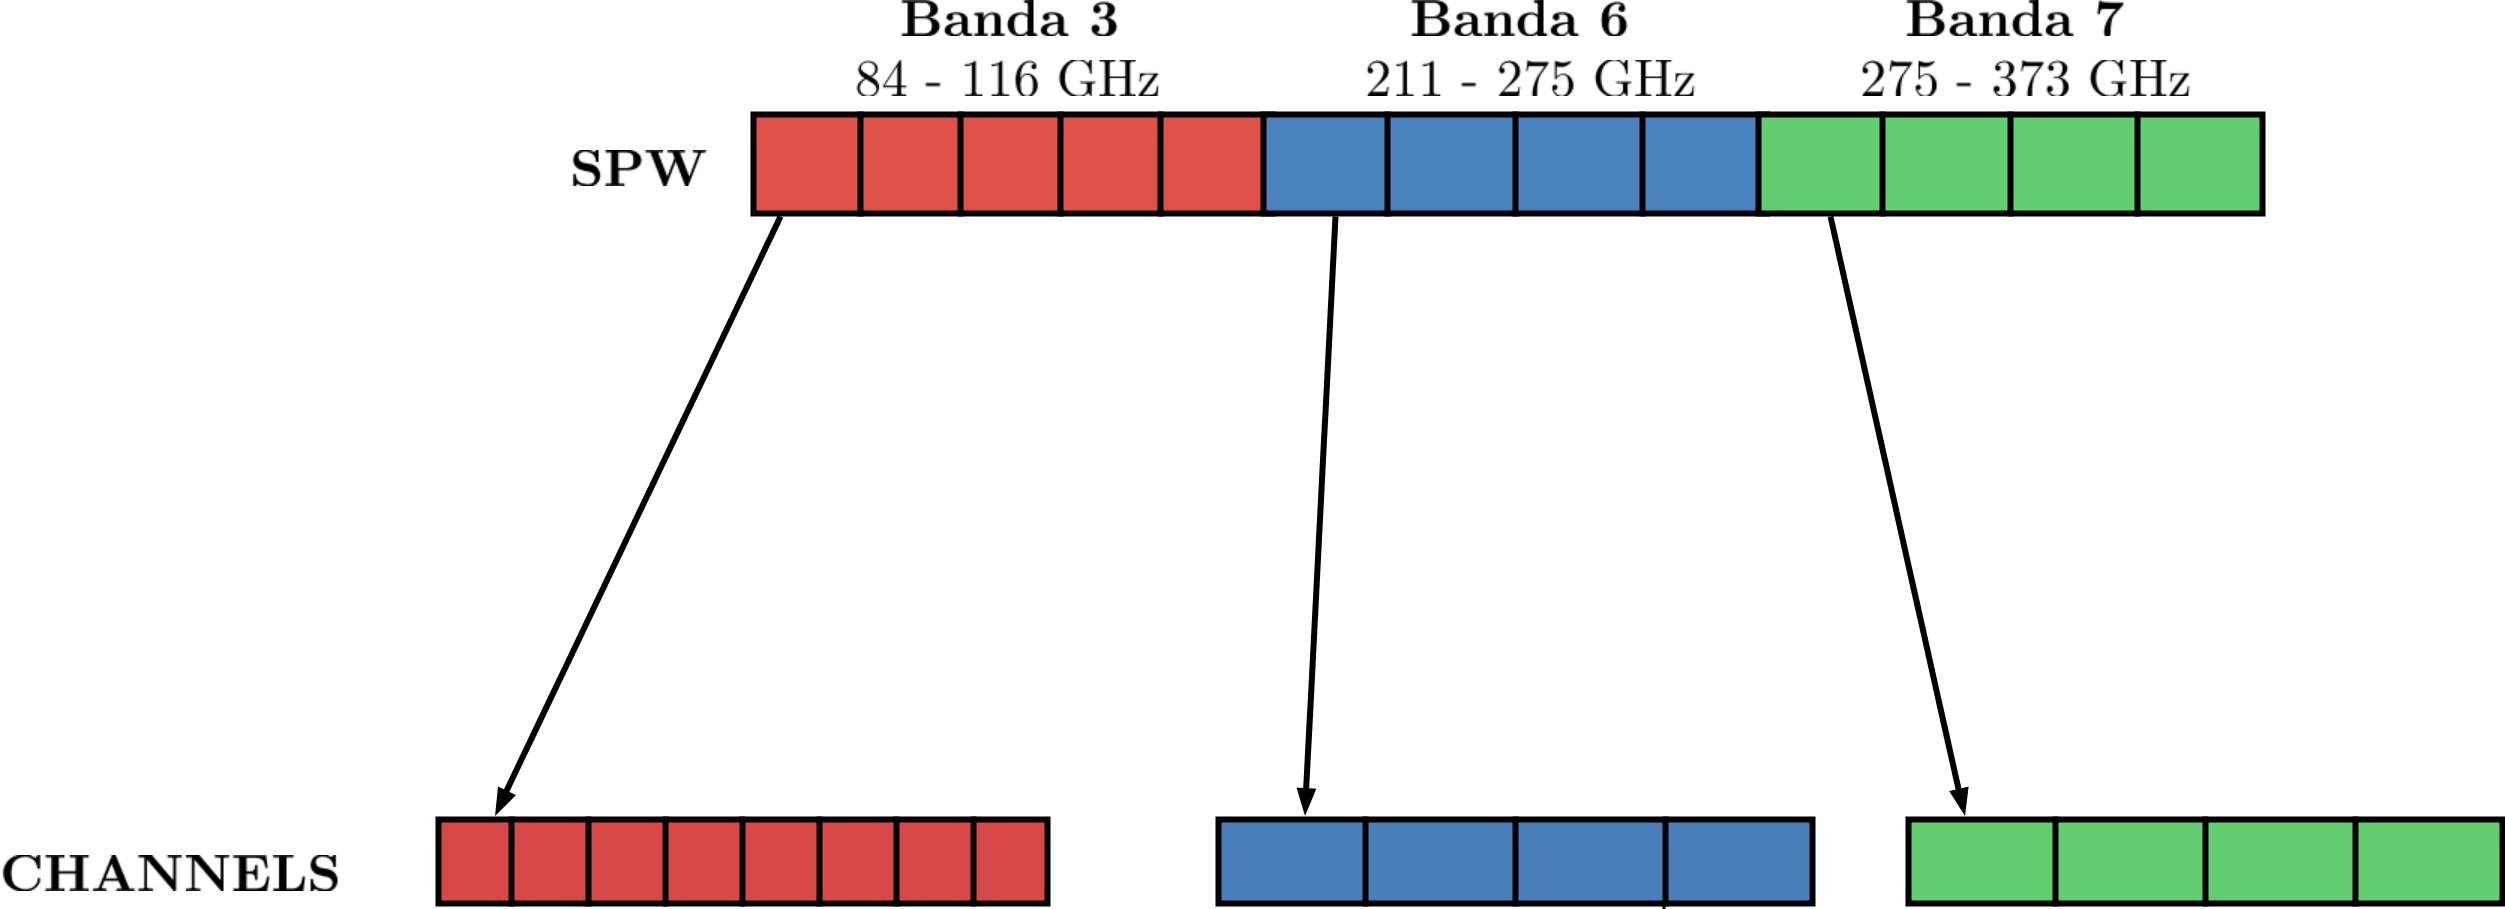
\includegraphics[scale=0.15]{images/frecuencias.png}
\caption{Bandas, \textit{spectral windows} y canales del objeto HL-Tauri. Fuente: Elaboración propia}
\label{fig:division}
\end{figure}

   


Luego de que las ondas milimétricas y submilímetricas son recibidas por las antenas, éstas deben ser discretizadas y procesadas en uno de los dos correlacionadores. El correlacionador \textit{64-input} es usado principalmente por los conjuntos de antena de 12 metros, mientras que el correlacionador ACA es usado por las antenas de 7 metros que componen el \textit{Atacama Compact Array}. Así, ambos correlacionadores funcionan simultáneamente e independientemente, por lo que mientras las antenas de 12 metros pueden estar observando un objeto y usan el correlacionador \textit{64-input}, las antenas de 7 metros pueden estar observando el mismo y otro objeto, y además, usando el correlacionador ACA \citep{alma-handbook}. 

Es importante destacar que los correlacionadores reciben señales de voltaje desde cada antena, calculan la correlación cruzada y autocorrelación para éstas por cada par de antenas (\textit{baselines}), y producen las visibilidades de valores complejos que los astrónomos reciben para sintetizar imágenes. Para entender de mejor forma qué son las visibilidades y cual es la implicancia que tienen en la síntesis de imágenes es necesario conocer los conceptos esenciales de interferometría.

\section{Principios y conceptos de interferometría}

La interferometría es una técnica usada para obtener imágenes de alta resolución angular de un fenómeno astronómico particular. Esta implica la combinación de señales recibidas desde el cielo por dos antenas separadas físicamente. Estas señales contienen ruido, permitiendo así que la distribución del brillo del cielo sea muestreada en una escala angular más pequeña que la de una sola antena. 

La resolución angular de un interferómetro, $\delta$, es el ángulo más pequeño en el que dos objetos pueden ser separados en orden de distinguirlos como objetos diferentes. Usando la teoría de la difracción, se puede demostrar que que para un interferómetro circular en particular de diámetro $D$, y una radiación de longitud de onda $\lambda$, este valor es $\delta \propto \frac{\lambda}{D}$. Esto quiere decir, que para grandes longitudes de onda (pequeñas frecuencias), se necesita un gran telescopio para obtener una buena resolución. Sin embargo, existen límites prácticos para construir un telescopio de un gran tamaño. Es por ello que haciendo uso de un conjunto de interferómetros situados a una distancia $D$, es posible obtener la misma resolución que un solo telescopio de radio $D$.



La relación entre la distribución del brillo del cielo y una visibilidad compleja está dada por el teorema de van Cittert-Zernike \citep{zernike} y es la base de la interferometría. Dado que los interferómetros no obtienen la imagen del cielo directamente, sino que obtienen visibilidades, que son que son la transformada de Fourier de la distribución del brillo del cielo en el plano de la imagen. Cada par de antenas forma un vector $\vec{k} = (u,v)$ en el plano de Fourier. Así mismo, la distribución del brillo del cielo es la transformada inversa de Fourier de las visibilidades complejas. Por lo tanto, la visibilidad $V(\vec{k})$ para un par de antenas con un \textit{baseline} $\vec{k}$, y su respectiva transformada inversa es:

%\begin{equation}
%V(\vec{k}) = \int_{-\infty}^{+\infty} A(\vec{x})I(\vec{x})e^{2\pi i %\vec{k}\vec{x}}\frac{dx dy}{\sqrt{1-x^{2}-y^{2}}}
%\end{equation}

\begin{align}
V(\vec{k}) &= \int\int A(\vec{x})I(\vec{x})e^{-2\pi i\vec{k}\vec{x}}dxdy \\
A(\vec{x})I(\vec{x}) &= \int\int V(\vec{k})e^{2\pi i\vec{k}\vec{x}}dudv
\end{align}

Donde $\vec{x} = (x,y)$ son las coordenadas del objeto a observar y estudiar, $A(\vec{x})$ es el \textit{primary beam}, $I(\vec{x})$ es la intensidad del objeto en $\vec{x}$, y $\vec{k}$ es el vector que se forma por cada par de antenas. 

\begin{figure}[h!]
\centering
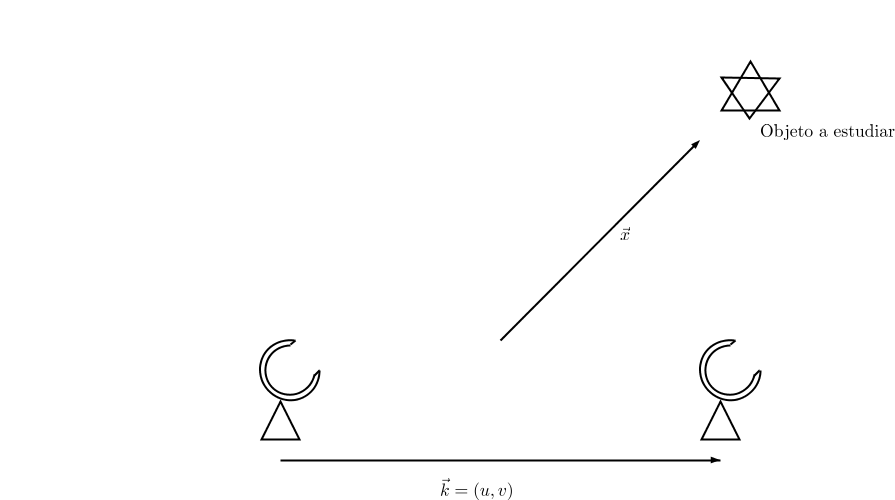
\includegraphics[scale=0.4]{images/antenas.png}
\caption{Dos antenas y su respectivo \textit{baseline}. $\vec{x}$ es la posición del objeto estudiado, y por otro lado $\vec{k}$ es el \textit{baseline} correspondiente a las dos antenas. Fuente: Elaboración propia.}
\label{fig:antena}
\end{figure}

Esto quiere decir que la imagen de la distribución del brillo del cielo puede recuperarse a través del muestreo de la distribución de visibilidades complejas en el plano $(u,v)$. En esencia, una imagen es la transformada de Fourier de las visibilidades donde cada una de éstas tiene una amplitud y una fase representando el brillo y la posición relativa de la emisión en una escala angular específica.

%Debido a que existe un número finito de pares de antenas, al llevar a cabo una transformada de Fourier inversa aparecen \textit{side-lobes} rodeando al \textit{primary beam}. Los \textit{side-lobes} son irregularidades en los patrones de radiación debido a la extensión finita de los puntos en el plano $(u,v)$ y a deficiencias en la cobertura. La transformada inversa de Fourier aplicada a las visibilidades es llamada \textit{dirty map}. El \textit{dirty map} ($I_{D}$) es la imagen del cielo ($I_{sky}$) convolucionada con el \textit{beam} del interferómetro ($B$).

%\begin{equation}
%I_{D} = I_{sky} \ast B
%\end{equation}  

%El \textit{beam} $B$ para un interferómetro con un conjunto de \textit{baselines} $\{\vec{k}_{k}\}$ puede ser representado por la transformada inversa de Fourier de una suma de diferencias en estos puntos en el plano $(u,v)$. 

%\begin{align}
%B(\vec{x}) &= \int_{-\infty}^{+\infty}\sum_{k}\delta(\vec{k}-\vec{k}_{k})e^{2 \pi i \vec{k}_{k}\vec{x}}dudv \\
%&= \sum_{k}\left(\cos(-2\pi\vec{k}_{k}\vec{x})+i\sin(-2\pi\vec{k}_{k}\vec{x})\right) \\
%&= \sum_{k}\cos(2\pi\vec{k}_{k}\vec{x})
%\end{align}


Los datos astronómicos resultan desde la adición de el ruido instrumental hasta la convolución de la imagen del cielo con la respuesta instrumental. Debido al muestreo incompleto en el plano $(u,v)$, la obtención de una imagen del cielo se convierte en un problema inverso que requiere algoritmos de síntesis de imágenes. 


\section{Métodos existentes de deconvolución} 

\subsection{CLEAN}

Uno de los algoritmos más exitosos y utilizados por la comunidad astronómica es CLEAN, creado por \citep{hogbom}. CLEAN postula que la distribución de intensidad está compuesta de fuentes puntuales. Dado que la imagen de una fuente puntual está dada por la convolución de ésta con el \textit{dirty beam} o Point Spread Function (PSF) (Ecuación \ref{eq:dirtybeam}). Donde este último está dado por:

\begin{equation}
B(x,y) = \int\int S(u,v) \exp\{2\pi j(ux+vy)\} \;du\,dv
\label{eq:dirtybeam}
\end{equation}

En cada iteración CLEAN encuentra el punto más brillante en la \textit{dirty image} (Ecuación \ref{eq:dirtyimage}) que está dada por:

\begin{equation}
I_{D}(x,y) = \int\int V(u,v)S(u,v)e^{2\pi i(ux+vy)}\;du\,dv
\label{eq:dirtyimage}
\end{equation}

Donde,

\begin{equation}
I^{T}(x,y) = \int\int V(u,v)e^{2\pi i(ux+vy)}\;du\,dv
\label{eq:fullcoverage}
\end{equation} 

Y luego por el teorema de la convolución se tiene que:

\begin{equation}
I_{D}(x,y) = I^{T}(x,y) \ast B(x,y)
\end{equation}

CLEAN agrega este punto (posición e intensidad) a la lista de fuentes puntuales. Luego, una fracción de ésta ($\gamma$, $0 < \gamma < 1$) es removida de la \textit{dirty image} y de las visibilidades. Este proceso se repite hasta que la imagen residual ($I_D$) sea solamente ruido.

Finalmente se calcula la imagen reconstruida convolucionando la lista de fuentes puntuales con el \textit{beam} de CLEAN, que se asume la mayoría de las veces como una Gaussiana.

\begin{algorithm}
\begin{algorithmic}[1]
    \STATE{Compute $I_D(x,y)$}
    \STATE{$B_R(x,y) = Gaussian$}
    \STATE{$i=0$}
    \WHILE{$I_D$ not noise-like}
        \STATE{$(x_i, y_i) = \arg\max I^D(x,y)$}
        \STATE{$\lambda_i = I(x_i, y_i)$}
        \FORALL{$(u,v)$}
            \STATE{$V(u,v) -= \gamma \lambda_i \exp\{-2\pi j(u x_i+ v y_i)\}$}
        \ENDFOR
        \STATE{Recompute $I_D(x,y)$}
        \STATE{$i=i+1$}
    \ENDWHILE
    \STATE{$I_R(x,y) = I_D(x,y) + \sum_i \gamma\lambda_i B_R(x-x_i,y-y_i)$}
\end{algorithmic}
\label{alg:clean}
\caption{Algoritmo CLEAN}
\end{algorithm}


\subsection{MEM Mono-frecuencia}


El método de máxima entropía (MEM) encuentra la imagen que simultáneamente se ajuste mejor a los datos, dentro de un nivel de ruido y que maximice la entropía $S$. Esto se lleva a cabo minimizando la función:

En MEM, la imagen y los datos son considerados variables aleatorias con distribuciones de probabilidad conocidas.

Sea $P(V|I)$ la probabilidad de ver las visibilidades $V$ dada la imagen $I$ y sea $P(I)$ un conocimiento \textit{a priori} de la imagen. Entonces mediante el teorema de Bayes se obtiene:

\begin{equation}
P(I|V) = \frac{P(V|I)P(I)}{P(V)}
\label{eq:bayes}
\end{equation}	

La probabilidad $P(V|I)$ puede ser aproximada mediante el hecho de que las visibilidades están corruptas por un ruido Gaussiano. Entonces dada la función modelo de visibilidades $V_{k}^{m}(I)$ y las varianzas observadas $\sigma_k$, la probabilidad puede modelarse como lo muestra la ecuación \ref{eq:chi2}, donde $V_{k}^{o}$ son las visibilidades observadas.

\begin{equation}
 P(V|I) \propto \exp\biggl\{-\sum_k^{Z}{\frac{|V^m_k(I)-V^o_k|^{2}}{\sigma_k^{2}}}\biggr\}
 \label{eq:chi2}
\end{equation} 

El \textit{prior} $P(I)$ se considera una distribución multinomial de una intensidad total discreta que cubre la imagen completa. Sea $n$ el número de píxeles y sea $N_{i}$ el número de fotones en el píxel $i$, el \textit{prior} puede expresarse de la forma:

\begin{equation}
P(I) = \frac{N!}{n^N\prod_i{N_i!}} 
\label{eq:imageProb}
\end{equation}

Donde $N=\sum_i N_{i}$ y la intensidad de la imagen en el píxel $i$ es interpretado en el modelo como $I_{i} \propto N_{i}$.

El término $P(V)$ en la ecuación \ref{eq:bayes} es independiente de $I$, por lo tanto no forma parte de la ecuación. Usando logaritmo y la aproximación de Stirling para factoriales y además omitiendo constantes aditivas relevantes el problema de reconstrucción de la imagen se convierte en la búsqueda de una imagen que satisfaga la probabilidad Maximum a Posteriori (MAP).

\begin{equation}
\arg \max_{I} \biggl\{
            -\frac{1}{2} \sum_k^{Z}{ \frac{|V^m_k(I)-V^o_k|^{2}}{\sigma_k^2} }-
            \lambda \sum_i^{n}{I_i \log{\frac{I_i}{G}}}
            \biggr\}
\label{eq:phi}
\end{equation} 

Se reconoce al primer término de la ecuación \ref{eq:phi} como $\chi^{2}$ y al segundo como la entropía de Shannon $S$. Estos dos parámetros son relevantes en el modelo, así como $\lambda$ que tiene un rol similar a los multiplicadores de Lagrange y actúa como un penalizador.

Finalmente, se cambia el signo de la ecuación \ref{eq:phi}, convirtiendo el problema en una minimización.

\begin{align}
\label{eq:phiFinal}
 \Phi = \frac{1}{2}\sum_k^{Z}{{\frac{|V^m_k(I)-V^o_k|^2}{\sigma_k^2}} + \lambda \sum_i^{n}{I_i \log{\frac{I_i}{G}}}}
\end{align}


Note que la Ecuación \ref{eq:phiFinal} es no lineal, por lo que debe ser minimizada con los algoritmos apropiados, en el caso de la solución que se propone, el método usado es el del gradiente conjugado Polak-Ribiere \citep{polak}. Además, es importante destacar que esta ecuación asume la existencia de un \textit{spectral window} y un solo canal.

En el Anexo \ref{apendice:dphi} se adjunta el cálculo del gradiente de esta función.
\subsection{MEM Multi-frecuencia}










%\chapter{GPGPU}
%\label{cap:gpgpu}

%\section{Arquitectura Unificada de Dispositivos de Cómputo}
%\subsection{Arquitectura}
%\subsection{cuFFT}
%\subsection{Peer-to-Peer}
%\subsection{Acceso virtual unificado}
%\subsection{GPUVMEM}

%\chapter{MEM Multi-frecuencia}
\chapter{Pruebas}
\label{cap:pruebas}

\chapter{Resultados}
\label{cap:resultados}
